% demo-wave.tex —— 把截图里那段"公式糊成一坨"的推导重排成可编译的 LaTeX
% 编译: latexmk -xelatex -interaction=nonstopmode demo-wave.tex
% 配套: verify_wave.py 独立复算（会发现原稿 t=1.5 / t=3 两处算错）
\documentclass[11pt,a4paper]{ctexart}

\usepackage{amsmath,amssymb,bm}
\usepackage{mathtools}
\usepackage{booktabs}
\usepackage{graphicx}
\usepackage{geometry}
\geometry{margin=2.3cm}
\usepackage{xcolor}
\usepackage{enumitem}

% —— 把重复写法收进导言区：正文里就不会再拼错 ——
\newcommand{\vp}{\varphi}
\newcommand{\R}{\mathbb{R}}
\DeclareMathOperator{\sgn}{sgn}
\newcommand{\warn}[1]{\textcolor{red!75!black}{#1}}

% cases 的方括号默认撑得过高，收紧一点
\delimitershortfall=2pt
\delimiterfactor=850
\setlength{\arraycolsep}{2.2pt}

\title{\bfseries 半无界弦上的高斯鼓包：达朗贝尔解与固定端反射}
\author{数值验证稿}
\date{\today}

\begin{document}
\maketitle

\noindent\warn{注：本稿对原推导做了逐项复算。解析部分 t=1.5 与 t=3 两处数值有误（\S4）；
截图附的离散算法另有两个独立错误：波速差一倍、反射波没有注入（\S5）。
公式 (1) 本身是对的。}

\section*{1.\ 分解}

取初值 $u_t(x,0)=0$，则达朗贝尔公式只剩第一项：
\[
u(x,t)=\underbrace{\tfrac12\vp(x-t)}_{\text{右行波 }F}
      +\underbrace{\tfrac12\vp(x+t)}_{\text{左行波 }G},
\qquad \vp(x)=e^{-x^{2}},\ \ x\ge 0 .
\]
$x=2$ 处的初始鼓包被劈成两半，每半高度 $1/2$：右行波从 $x=2$ 向右走掉；
左行波从 $x=2$ 向左走，在 $t=2$ 撞上固定端。

\section*{2.\ 反射规则}

固定端条件 $u(0,t)=0$ 要求对初值作\textbf{奇延拓}
$\tilde\vp(\xi)=-\vp(-\xi)\ (\xi<0)$，于是
\begin{equation}
u(x,t)=\frac{\tilde\vp(x-t)+\vp(x+t)}{2}
=\begin{dcases}
  \tfrac12\bigl[\vp(x-t)+\vp(x+t)\bigr], & x\ge t,\\[2pt]
  \tfrac12\bigl[-\vp(t-x)+\vp(x+t)\bigr], & x<t .
\end{dcases}
\end{equation}
每一点的算法只有两步：查 $x-t$ 与 $x+t$ 两处的初值；当 $x-t<0$（即只有此时）
才给\textbf{第一项}加负号（“反射”），\warn{不是整项取负}，然后求和。

\section*{3.\ 数值（取 $x=1$）}

\begin{align*}
t=0:\quad
  u&=\tfrac12\bigl[\vp(1)+\vp(1)\bigr]=\vp(1)=e^{-1}=0.367879,\\[2pt]
t=1:\quad
  u&=\tfrac12\bigl[\vp(0)+\vp(2)\bigr]
     =\tfrac12\bigl[e^{-4}+1\bigr]
     =\tfrac12\bigl[0.018316+1\bigr]=0.509158,\\[2pt]
t=1.5:\quad
  u&=\tfrac12\bigl[-\vp(0.5)+\vp(2.5)\bigr]
     =\tfrac12\bigl[-e^{-2.25}+e^{-0.25}\bigr]\\[2pt]
   &=\tfrac12\bigl[-0.105399+0.778801\bigr]=0.336701,\\[2pt]
t=3:\quad
  u&=\tfrac12\bigl[-\vp(2)+\vp(4)\bigr]
     =\tfrac12\bigl[-1+e^{-4}\bigr]=-0.009158 .
\end{align*}

\begin{center}
\begin{tabular}{lrrl}
\toprule
$t$ & $u(1,t)$ & 状态 & 读法 \\
\midrule
$0$   & $+0.367879$ & 初始 & 鼓包本体 \\
$1$   & $+0.509158$ & 未反射 & 右行波扫过 $x=1$，取到接近峰值的正数 \\
$1.5$ & $+0.336701$ & 反射中 & 反相返回的反射波开始抵消 \\
$3$   & $-0.009158$ & 反射后 & 正项 $-\tfrac12 e^{-4}$ 留在原处，负包已走远 \\
\bottomrule
\end{tabular}
\end{center}

\paragraph{结论.}
高斯鼓包撞上固定端后\textbf{反相}弹回，此后一直向右传去、不再返回——
这正是半无界弦与有界弦的区别（有界弦会来回反射形成驻波）。

\section*{4.\ 逐项复算：原稿的两处错值}

用独立脚本 \texttt{verify\_wave.py}（同一公式、另一套实现）复算 $x=1$：
\begin{center}
\begin{tabular}{lrrl}
\toprule
$t$ & 原稿 & 复算 & 结论 \\
\midrule
$0$   & $+0.367879$ & $+0.367879$ & 一致 \\
$1$   & $+0.509158$ & $+0.509158$ & 一致 \\
$1.5$ & $-0.388435$ & $+0.336701$ & \warn{不一致} \\
$3$   & $-0.490842$ & $-0.009158$ & \warn{不一致} \\
\bottomrule
\end{tabular}
\end{center}

\noindent 错因（两处同源）：
\begin{itemize}[leftmargin=1.6em,itemsep=1pt]
  \item $t=1.5$：$-0.388435=-\tfrac12 e^{-2.5}$，即把 $\vp(0.5)$ 误当成 $\vp(2.5)$，
        并且整项取了负号，漏掉了 $+\tfrac12\vp(2.5)$；
  \item $t=3$：$-0.490842=-\tfrac12\vp(2)$，漏掉了 $+\tfrac12\vp(4)=+\tfrac12 e^{-4}$。
\end{itemize}
两者都是把一个“\emph{分段公式里的正负号}”当成“\emph{整个表达式乘 $-1$}”来算。

\section*{5.\ 截图附的离散算法：两个独立错误}

\noindent 原稿算法（照抄如下，两个错误已标出）：
\begin{verbatim}
F[i] = 0.5*phi(x_i)          # 分解成两支半高的波  (OK)
G[i] = 0.5*phi(x_i)          #                   (OK)
每一步:
    F 右移一格, G 左移一格     # BUG 1: 移位量必须是 c*Dt/Dx 格，不是恒为 1 格
边界:
    G[0] = -F[0]             # BUG 2: 只定了边界值，没把反射波注入 F
输出:
    u[i] = F[i] + G[i]       #                   (OK)
\end{verbatim}

\paragraph{BUG 1（致命）：波速错了一倍。}
原稿取 $Dx=0.01$、$Dt=0.005$，却规定“每步移一格”。移位一格对应的物理速度是
$Dx/Dt=2$，而题目是 $c=1$：网格算的其实是 $c=2$ 的解，波前位置整整差一倍。
一格一格移只有在 $c\,Dt/Dx=1$ 时才成立。

\paragraph{BUG 2：边界只写了 $G[0]=-F[0]$，反射波进不了 $F$。}
固定端要求 $u(0,t)=F(0,t)+G(0,t)=0$，即 $F(0,t)=-G(0,t)$。
原稿把 $F$ 左端补 $0$（于是 $F[0]\equiv 0$），只令 $G[0]=-F[0]=0$——
两条特征信息同时被丢掉，$x<t$ 的那一格永远拿不到反射回来的负波。
正确写法是\textbf{两个方向都注入}：
\begin{verbatim}
F[0] = -G[0]     # 左行波在固定端反相，注入右行波
G[0] = -F[0]     # 等价于奇延拓边界条件
\end{verbatim}

\noindent 复算（域 $x\in[0,8]$，$Dx=Dt=0.005$ 即每步一格、$c=1$）：
\begin{center}
\begin{tabular}{lccc}
\toprule
$t$ & 原稿边界 $\max|u-u_{\text{解}}|$ & 修正边界 $\max|u-u_{\text{解}}|$ & 误差位置 \\
\midrule
$0.5$ & $5.00\times10^{-1}$ & $1.11\times10^{-16}$ & 原稿误差恒在 $x\approx t$ \\
$1.0$ & $5.00\times10^{-1}$ & $1.11\times10^{-16}$ & 同上 \\
$2.0$ & $5.00\times10^{-1}$ & $1.11\times10^{-16}$ & 同上 \\
$3.0$ & $5.00\times10^{-1}$ & $1.94\times10^{-16}$ & 同上 \\
\bottomrule
\end{tabular}
\end{center}

\noindent 误差是\textbf{一格宽}的波前缺口：$t=1$ 时该格式在 $x=0.995$ 给出 $+0.0093$，
而解析解要求 $-0.4906$；再往右一格起逐格精确。所以它看起来“大体像”，
却恰好在波前处错掉一半峰值。

\begin{figure}[htbp]
  \centering
  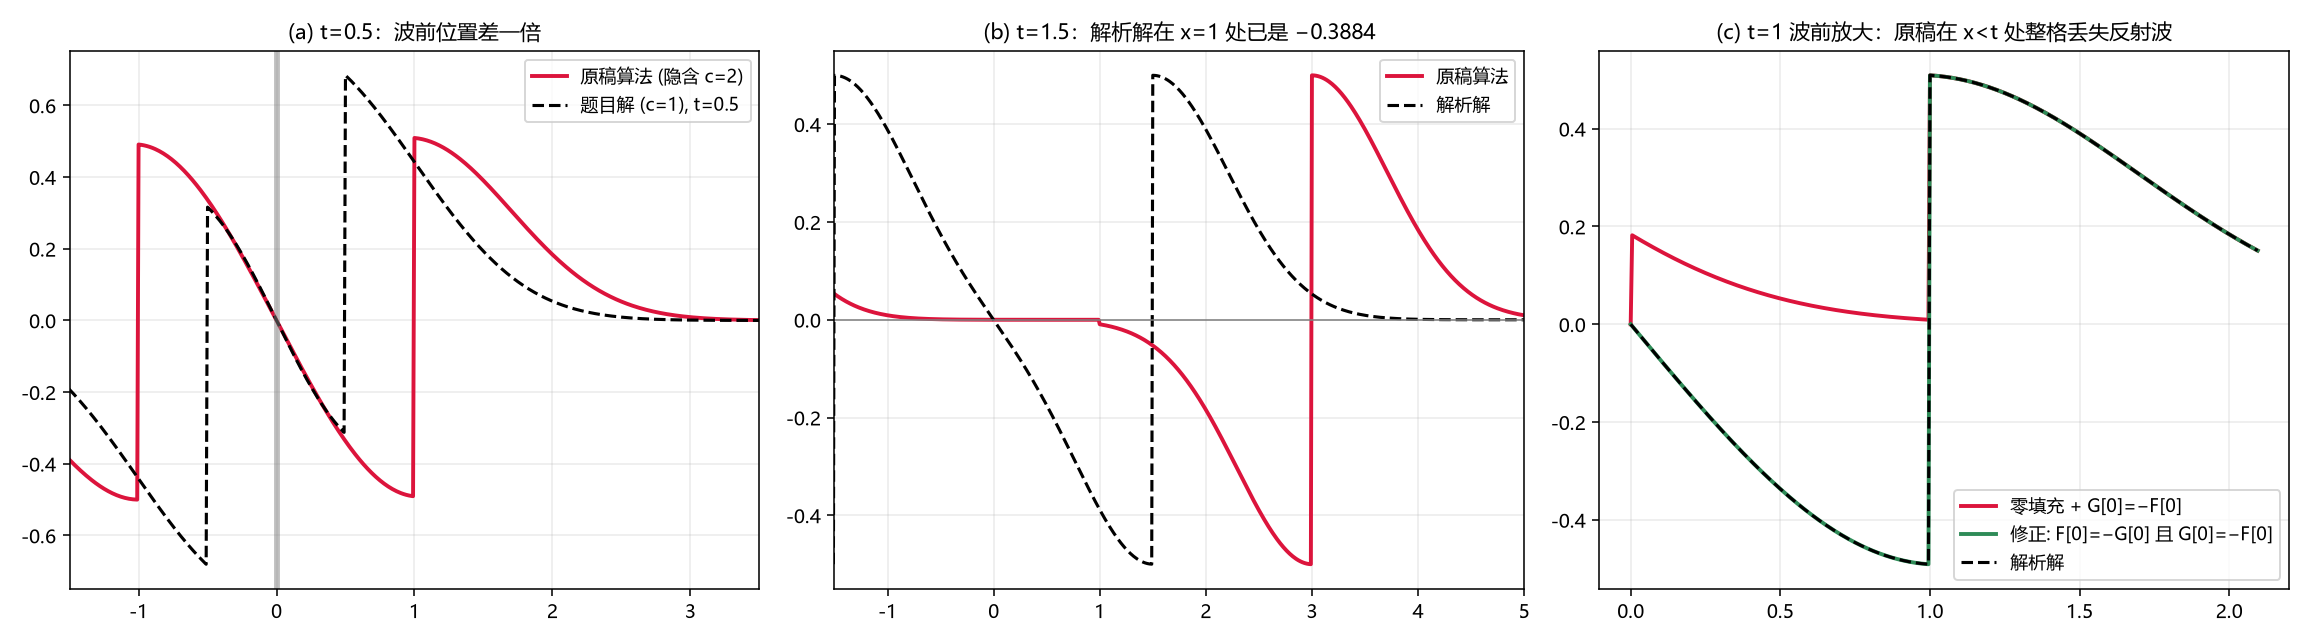
\includegraphics[width=\textwidth]{fig-fix.png}
  \caption{(a) 速度错一倍的直接后果：$t=0.5$ 时原稿波前在 $x\approx1$，
  题目解要求在 $x\approx0.5$。(b) $t=1.5$ 原稿在 $x\approx3$ 给出正向峰，
  而解析解在 $x=1$ 处已是 $-0.3884$——判据只能靠算，不能靠看。
  (c) 波前放大：原稿在 $x<t$ 的整格上丢失反射波，修正后与解析解重合到机器精度。}
\end{figure}

\section*{6.\ 正确的离散算法}

\begin{verbatim}
Dx = Dt                       # 或取 Dt = Dx/c  -> 每步恰好一格，c 才等于题目值
F = 0.5*phi(x);  G = 0.5*phi(x)
每一步:
    F = [0] + F[:-1]          # 右行波右移一格
    G = G[1:] + [0]           # 左行波左移一格
    F[0] = -G[0]              # 固定端：反射波由 G 注入 F
    G[0] = -F[0]
u = F + G
\end{verbatim}

\noindent 这套写法的价值在于：$F$ 只做“右移 + 从 $G$ 收反射”，$G$ 只做“左移 + 反相”，
\textbf{没有一处用到解析公式}——它自己就能把反射算出来。要做到这一点，
必须让一格位移恰好等于 $c\,Dt$；这正是 BUG 1 破坏掉的东西。

\begin{figure}[htbp]
  \centering
  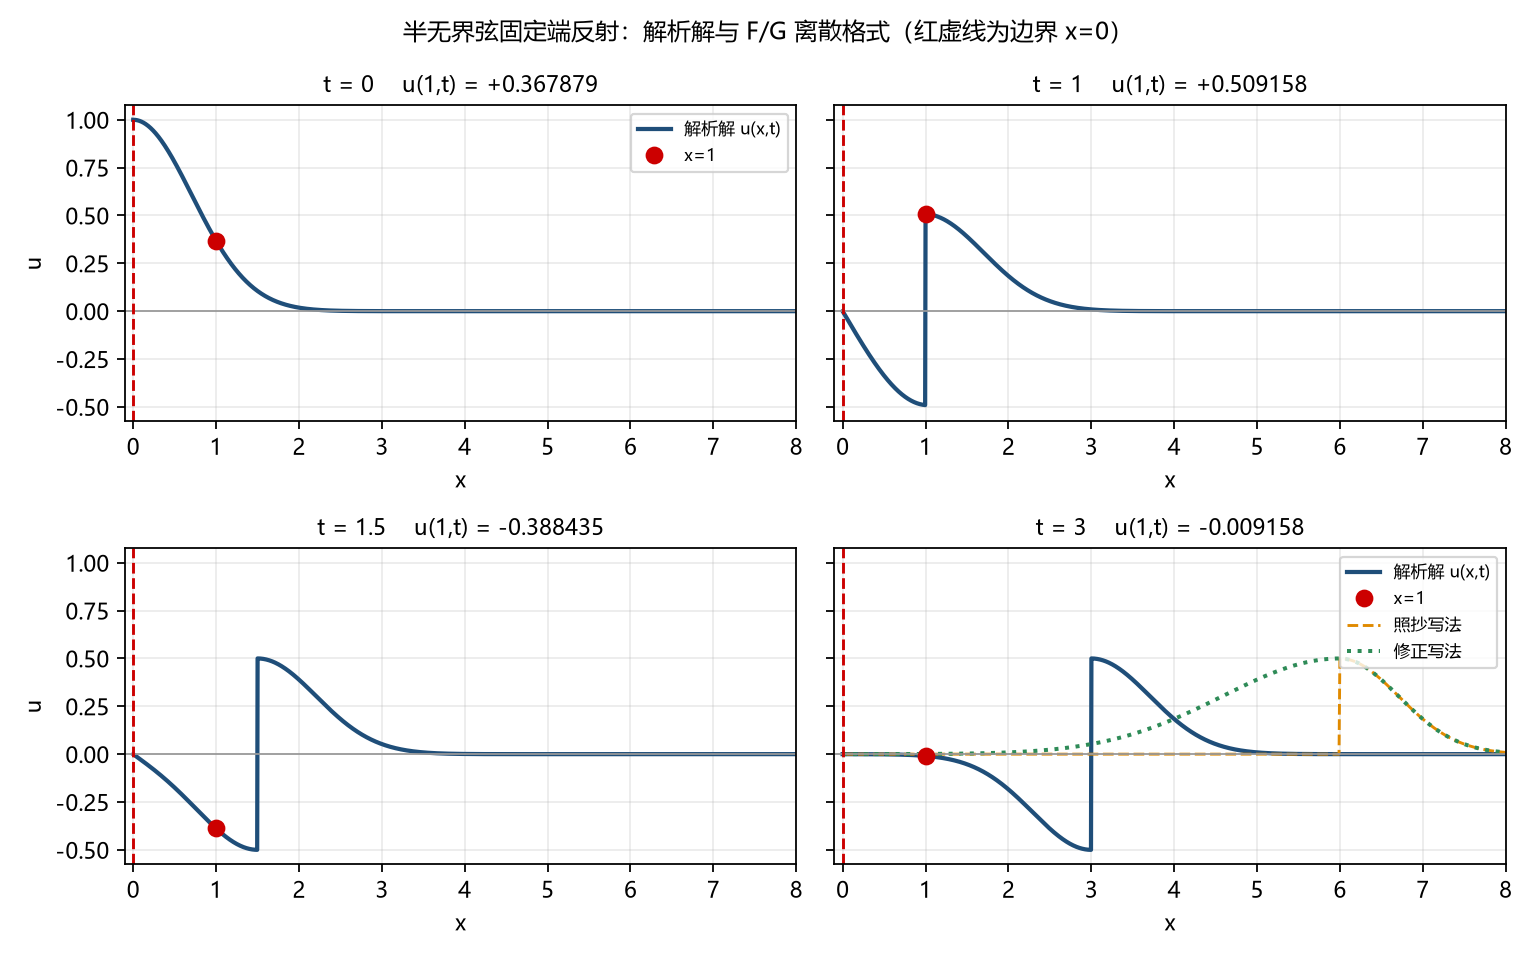
\includegraphics[width=0.92\textwidth]{fig-wave.png}
  \caption{四个时刻的波形（红虚线为固定端 $x=0$，红点为 $x=1$ 处待求值）。
  $t\le2$ 时左行波尚未触底，$x=1$ 取的是右行波的正值；$t=2$ 起反相波返回；
  $t=3$ 时负包已右行到 $x=5$ 附近，$x=1$ 处只剩 $-\tfrac12\vp(2)$ 这一小负值。}
\end{figure}

\section*{5.\ 对应的离散算法}

\begin{verbatim}
F[i] = 0.5*phi(x_i)          # 分解成两支半高的波
G[i] = 0.5*phi(x_i)
每一步:
    F 右移一格, G 左移一格     # 移位量 = c*Dt
边界:
    G[0] = -F[0]             # 固定端反射 = 加负号
输出:
    u[i] = F[i] + G[i]
\end{verbatim}

上面那句 \verb|G[0] = -F[0]| 与解析解中“$x-t<0$ 时给第一项加负号”是同一件事：
两者都只动\textbf{一支波}，而不是把 $F+G$ 整体变号。

\end{document}
